\subsection{Comments Upon Validity of Area Transformed Data}

gradient....

One method for converting each frame to an $\alpha$-value would have been to binarize and threshold its pixels, thereby counting the fraction of pixels deemed ``bright enough'' to be crystalline.  It was observed, however, that the 

\subsection{Comments Upon Accuracy of Grian-Counting Algorithm}

no attempt made to quantify accuracy, given that doing so would require training data using unknown parameters (local grain alignment, anisotropy, etc)...several regions of "miscounting/mislabling" were observed, and the degree of this depended heavily upon the defined parameters for the algorithm...suggested that the results of the algorithm only be viewed as correct in terms of a loose estimate, albeit a more rigorous way than counting by hand according to arbitrarily defined parameters; algorithm also inherently favors round grains, even though Te nuclei are quite anisotropic

FIGURE containing a region mislabled by the algorithm

	\begin{figure}[h]
		\centering
		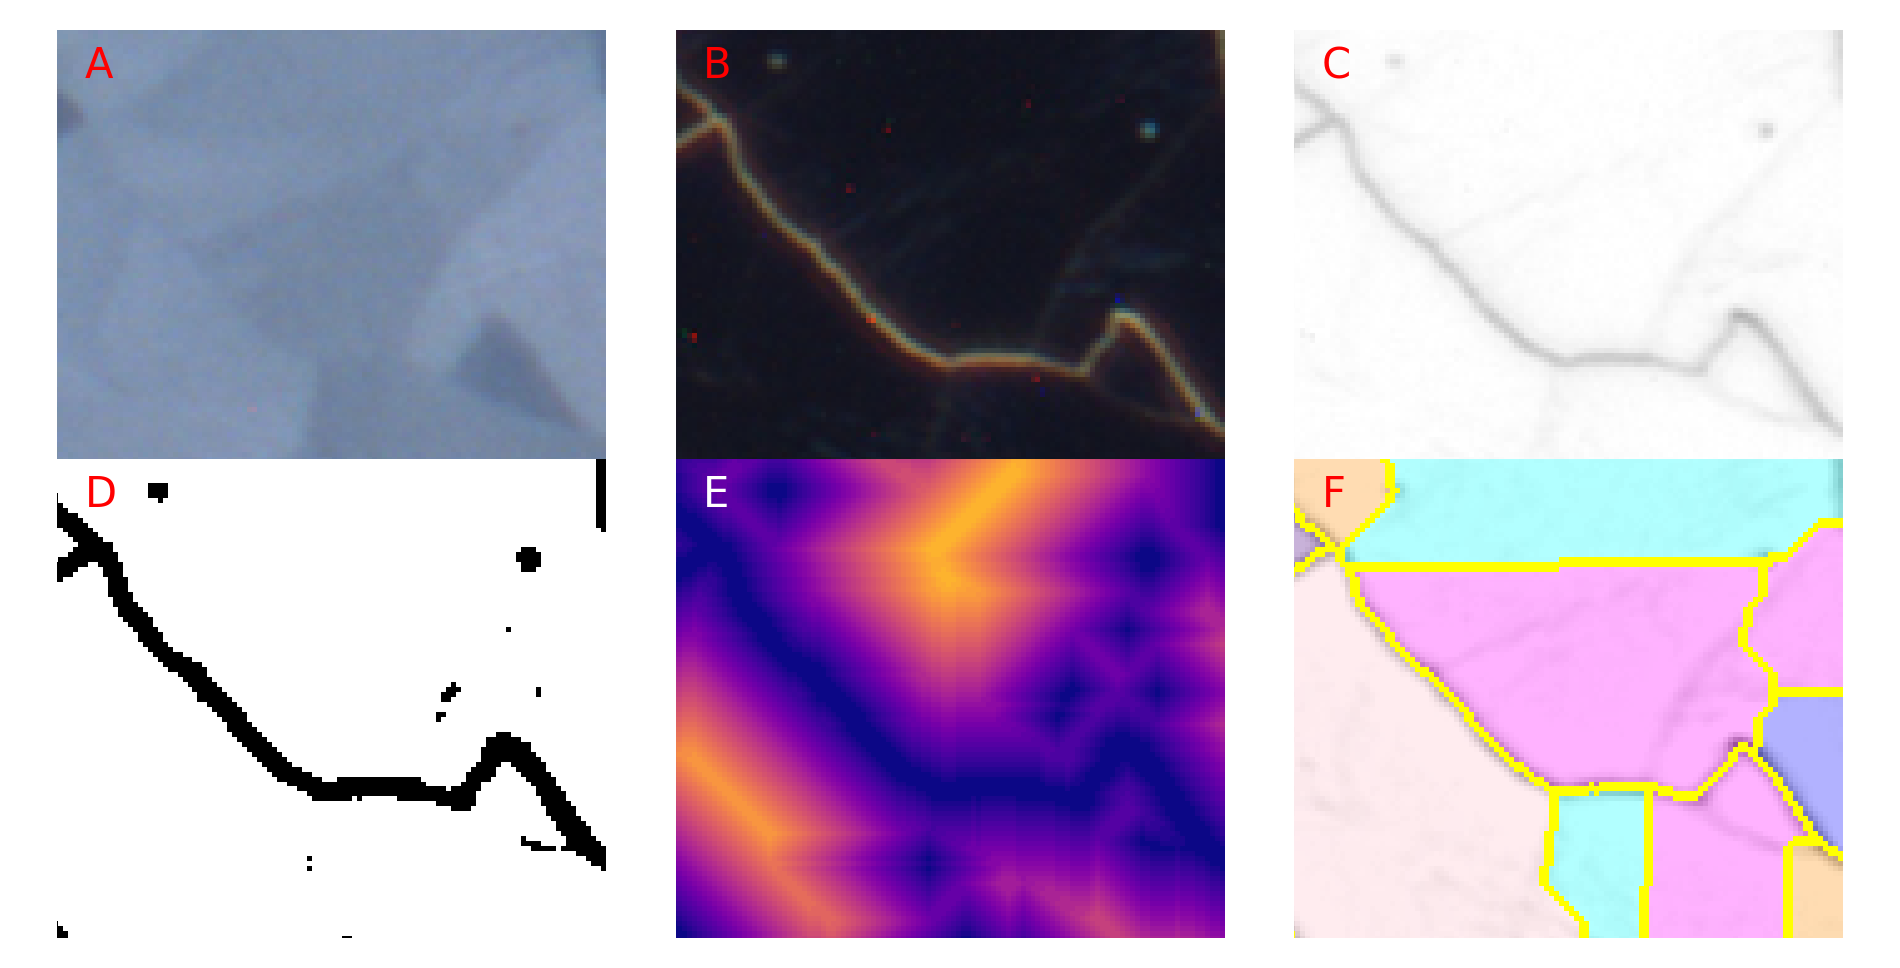
\includegraphics[width=1.0\linewidth]{miscount_10C.png}
		\caption{}
		\label{fig:miscount}
	\end{figure}

\subsection{Validity of Obtained Crystallization Parameters}

problem is that critical cluster size can be made arbitrarily large, and the author has not found any methodology for predicting the amorphous-crystalline surface energy...additional problem is that the nucleated grains are quite anisotropic, leading to different growth rates...therefore the critical size and the free energy difference should be taken with a grain of salt, though the nucleation and growth parameters look okay

it should be mentioned that, in theory, one could calculate gamma from B-D and JMAK theory...doing so requires a model for the fraction of surface atoms as a function of the atoms in the nucleus, and depends on the prefactors with their enormous uncertainty, which precludes this...an attempt was made albeit with unphysical results

\subsection{Areas of Improvement for Future Calculations}

change nuclei shape

perform MD simulations in order to generate better training data for the grain algorithm, following a similar protocol to that discussed in (ML paper)

perform MD simlations to model the interface energy and better estimate its magnitude?
